\section{The recovery curve could not see the estimator}
\label{sec:blind}

An earlier internal report validated the cutpoint on real held-out cells and
concluded it was sound. The statistic it used was a recovery curve: generate
samples with known composition and a known shift, run the estimator, plot
recovered against true. Ours ran between 1.00 and 1.07 wherever the rule said
``estimate'' on the reference draw --- 0.86 to 1.18 on the pooled one --- and
tightened with $n$ on both (\iffull Fig.~\ref{fig:generator}\else Appendix
Fig.~\ref{fig:generator}\fi). That is what a
working estimator looks like.

It is also what this one looks like with the estimator divided out. The
estimator in that arm applies Equation~\ref{eq:kitagawa} to the sample's
\emph{own} realised summary statistics, so it reproduces them exactly. Across
all 1{,}711{,}200 replicates of four sweeps on two cohorts,
$\max|\hat{\imath} - i_{\text{realised}}| = 0$. The ratio is therefore
$i_{\text{realised}} / i_{\text{parametric}}$: what the generator drew over what
it was asked for. No calculation beyond that reference remains in it.

\iffull
\begin{figure}[t]
\centering
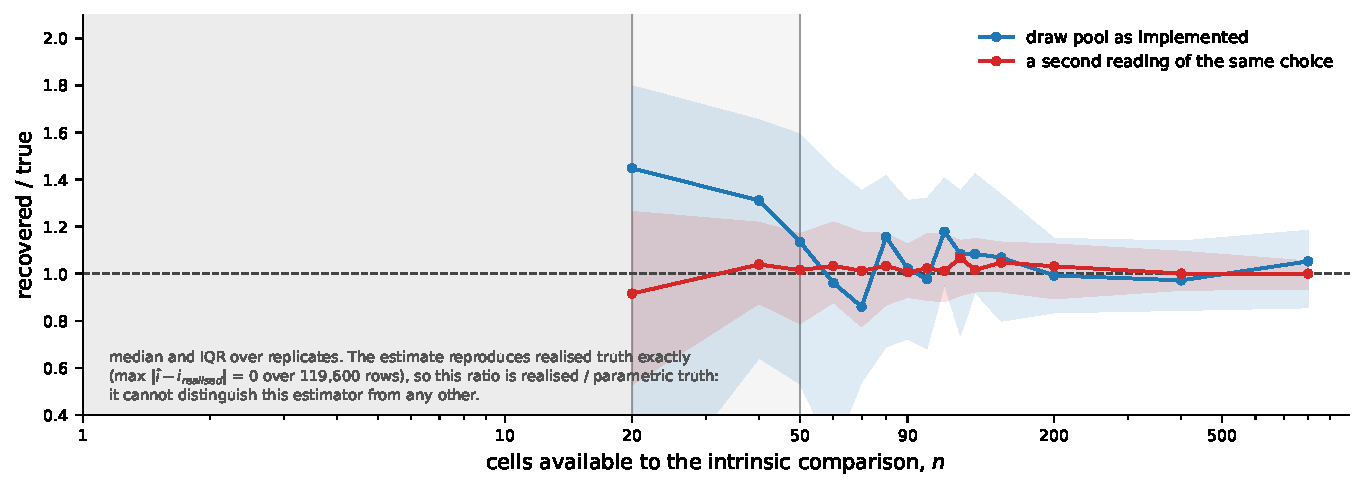
\includegraphics[width=\linewidth]{figures/fig3_generator_statistic.pdf}
\caption{Ratio of recovered to true intrinsic effect, median and IQR over 50
replicates at the detectable effect, for both draw pools. An earlier internal report used this curve to
conclude the committed cutpoint was ``validated on real cells''. The curve
behaves well wherever the rule says ``estimate'', and on this arm adds no validation beyond reproduction of the reference. The single-cell estimate applies
\texttt{decompose()} to the sweep's own realised summary statistics and
reproduces them exactly, with
$\max|\hat{\imath} - i_{\text{realised}}| = 0$ over all 119{,}600 replicates of
the sweep plotted here, and over all 1{,}711{,}200 of four sweeps on two
cohorts, leaving the ratio equal to
$i_{\text{realised}}/i_{\text{parametric}}$. A further 29{,}900 replicates
of \emph{this} sweep carry no ratio at all, and 427{,}800 across the four: at
$s = 1$ the parametric intrinsic term is exactly zero,
so the design's own null control is the one point where this validation
statistic cannot be evaluated. The statistic still
discriminates an estimator failing to reproduce its input, and the design
document ships a broken-estimator control returning $0.0$ for which the ratio
comes out zero. The oracle arm by construction is not such an estimator, so
validating it here is circular. The value at the zero-cell grid point ($f_T = 0$, where no mature
tumour cell survives and the rule abstains), read at the time as a two-fold
over-estimate in the dangerous direction, is exactly $1/(1-s)$: the realised
and requested mature fractions agree there, so the closed form carries no
scale factor.}
\label{fig:generator}
\end{figure}
\fi

\paragraph{The general form.} Let $D$ be a simulated draw requested at
$\theta$, and specify an observed-data reference $T(D)$ before comparing
estimators. We call $T(D)$ the realised reference, written
$\theta_{\text{realised}}$; it is not necessarily a realised causal effect.
Suppose $T(D)=h(S(D))$ and $\hat\theta(D)=h(S(D))$ for the \emph{same}
functional $h$ and summaries $S$. Then, for $\theta\ne0$,
\begin{mdframed}[linewidth=0.5pt,innertopmargin=4pt,innerbottommargin=4pt,%
  nobreak=true]
\[
\frac{\hat\theta}{\theta} \;=\; \frac{\theta_{\text{realised}}}{\theta}
\]
\begin{center}
\texttt{r = est - truth\_realised}\\
\texttt{assert not np.allclose(r, 0.0, atol=tol)}
\end{center}
\end{mdframed}
Sharing sufficient statistics alone is insufficient: different functions of the
same summaries need not agree. The assertion screens for numerical equality on
valid draws; only an algebraic argument establishes an identity. Under
consistency for nonzero $\theta$, this ratio approaches 1 as sampling error
shrinks.

\textbf{Equality identifies redundancy, not an invalid estimator.} The curve
still measures this functional's sampling performance relative to $\theta$.
It cannot distinguish algebraically equivalent implementations, or by itself
validate interval coverage or an abstention threshold. Even a correctly
implemented sample mean equals its empirical-mean reference. We use ``blind''
only for this redundancy relative to a specified reference, not as a verdict
on statistical validity.

\paragraph{The procedure, in four steps.} Everything after this paragraph is
evidence that the four steps are necessary. They are the contribution; run them
on the sweep you already have.

\begin{mdframed}[linewidth=0.5pt,innertopmargin=4pt,innerbottommargin=4pt]
\begin{enumerate}\itemsep1pt\parskip0pt\topsep2pt
\item \textbf{Pre-specify the reference $T(D)$} --- its functional form, its
      target population and its observation process --- \emph{before} the sweep
      runs. Which estimators the screen can see depends on this choice, so
      choosing it afterwards chooses the answer.
\item \textbf{Screen for equality.} Report
      $\max_D |\hat\theta(D) - T(D)|$ per design cell, not a pooled median, with
      \texttt{tol} set explicitly in outcome units. Count non-finite outputs
      separately: a NaN makes the assertion pass.
\item \textbf{Read an exact zero as redundancy, not as failure.} It proves the
      recovery ratio is a functional of the generator; it is not a verdict on
      the estimator. A nonzero residual certifies nothing on its own.
\item \textbf{Report scale beside the equality screen.} Give the residual in
      units of the generator's own sampling error, so a residual that is nonzero
      but small relative to that error is visible as such.
\end{enumerate}
\end{mdframed}

\noindent Step 1 is the one that is skipped, and Table~\ref{tab:matrix} is why it
matters: the same estimator reads blind or informative depending on which
reference was named. At a null requested effect, use differences rather than
recovery ratios.

\paragraph{How this wiring arose.} Our oracle arm used the summaries already
computed for the draw. This is an observed failure in our pipeline, not an
estimate of its prevalence in virtual-control-arm practice. The patient
examples below establish possibility across methods and designs, not frequency.

\paragraph{What this looks like in a trial simulator.} Consider a patient
simulator with treatment assignment and outcomes within covariate strata.
For stratum counts $n_g$, total $n$, and observed arm means $\bar Y_{ag}$, define
\[
T(D)=\sum_g\frac{n_g}{n}(\bar Y_{1g}-\bar Y_{0g}).
\]
Saturated G-computation \citep{robins1986} computes this reference directly.
IPW with empirical propensities $\hat p_g=n_{1g}/n_g$ does too: each stratum's
treated weighted sum divided by $n$ is $(n_g/n)\bar Y_{1g}$, and likewise for
controls. This requires nonempty arms within each stratum and these weights;
it is not an equivalence for arbitrary G-computation or propensity models.
The reference is an observed contrast, not the finite-sample average of paired
potential-outcome differences. Sharing a population outcome model alone does
not imply its exact reproduction.

\paragraph{So we built one.} Describing the fix is not demonstrating it, so
Figure~\ref{fig:trial} runs that simulator: three covariate strata, treatment
assigned with a stratum-dependent probability so the strata confound, a
requested effect of $\theta = 3$, and five estimators of it over cohorts from
100 to 5{,}000 patients.

Four of the five sit near 1 and tighten with cohort size --- the picture of a
validated estimator. Two of those four are exactly blind. G-computation over
the generator's own strata returns the realised effect with
$\max|\hat\theta - \theta_{\text{realised}}| = 0$, as the algebra says it must.
\textbf{So does inverse-probability weighting with a saturated propensity
model.} Their equivalence is algebraic, but a recovery curve alone does not expose
that equivalence as directly as the residual column.

Cross-fitting the IPW propensity \citep{chernozhukov2018} breaks it here. Fit the propensity on one fold and
apply it to the
other, so the weights on a patient come from data that patient is not in, and
the estimator becomes a different functional: still consistent, still sitting
near 1, but now with a residual that is non-zero at every cohort size and shrinks
as the estimate improves. That residual establishes departure from this reference, not validity.\iffull{} The unadjusted
difference is there to show the curve is not useless --- it ignores the strata,
so it is confounded, and the curve catches it immediately at a ratio near 2.4.\fi

\iffull
\textbf{Nothing has to be held out for the check to stay silent, though.} Cross-fitting
breaks the degeneracy by splitting the sample, which leaves the reading that the
residual merely notices folds. It does not. Ordinary least squares of the
outcome on treatment and additive stratum dummies --- the estimator most people
would actually write --- sees every record and splits nothing, and is correctly
specified here, since the effect is additive and homogeneous. It is still not the
generator's functional: standardisation weights each stratum by its prevalence
and OLS uses normalised weights proportional to
$n_g\,\hat p_g(1 - \hat p_g)$, with empirical $\hat p_g$, and the propensities differ across strata. Its residual is
non-zero at every cohort size, and \emph{smaller} than cross-fitted IPW's, so
the non-degenerate comparison here is not the weaker estimator. What the check
detects is a shared functional, not a shared sample --- and the two estimators
that look like careful causal inference are the blind ones.
\fi

\iffull
The lesson is not that oracle arms are bad. It is that \emph{near 1 and
tightening} is compatible with the estimator having been divided out, and that
the residual against realised truth is what separates the two.
\fi

\iffull
\paragraph{The check is sound and not complete, and we can say how incomplete.}
An identity proves redundancy: if $\hat\theta \equiv \theta_{\text{realised}}$
the ratio is a functional of the generator, by algebra. The converse fails, in
three ways we can measure (Table~\ref{tab:matrix}, 14 estimators $\times$ 3
designs $\times$ 2 realised truths $\times$ 6 cohort sizes $\times$ 6 seeds).

\textbf{Degeneracy belongs to the \emph{pair}, not the estimator.} OLS on
stratum dummies has residual $0.0663$ against the standardised realised truth
and reads informative. Against the variance-weighted realised truth --- the observed-data functional
equal to OLS by Frisch--Waugh --- it is
$3.5\times10^{-14}$, exactly blind. The swap runs both ways: G-computation is
$0$ against the first and $0.0663$ against the second. Our Table~\ref{tab:trial}
reports OLS as the row that sees the estimator; it departs from that reference, although both consistently estimate the
requested homogeneous effect.

\textbf{The verdict flips with the trial design.} Under our stratified
permuted-block randomisation with complete blocks and 1:1 allocation, empirical
propensities are $0.5$ by construction, the two reference functionals
coincide, and everything except cross-fitted IPW and finite-ratio matching sits
at machine zero: OLS $1.6\times10^{-14}$, and even the unadjusted difference
$6.7\times10^{-15}$. No estimator changed.

\textbf{Two more estimators are secretly the same functional.} AIPW with
saturated nuisances and no cross-fitting is $4.4\times10^{-15}$: the
augmentation term is identically zero within each stratum, so this
doubly-robust implementation collapses onto standardisation. Cross-fitting is
not necessary to avoid this identity; changing nuisance specifications can also
change the functional. Our cross-fitted comparison is IPW, not AIPW. Exact matching on
stratum is $8.9\times10^{-16}$ with all controls, $0.052$ at 20 and $0.164$ at
1 --- blindness set by a matching ratio nobody thinks of as a validation
choice. IPW with an $L_2$-penalised logistic propensity runs $0.403$, $0.045$,
$0.0103$, $0.010$ as $C$ goes $0.1, 1, 100, 10^6$, and $1.3\times10^{-6}$ once
the solver tolerance is tightened: five orders of magnitude of apparent
informativeness from a regularisation constant.

\paragraph{Report scale alongside the equality screen.} Put the residual in units of the
generator's own sampling error,
\[
\rho \;=\; \frac{\mathrm{med}\,|\hat\theta - \theta_{\text{realised}}|}
                {\mathrm{med}\,|\theta_{\text{realised}} - \theta|},
\]
a ratio of median absolute departures, not a fraction of the curve's spread.
OLS scores $\rho$ between $0.129$ and $0.137$ at every cohort size from
100 to 5{,}000, with no trend in $n$. The table's descriptive transform
$q=1/(1+\rho)$ is $88\%$ at the largest cohort; this is not a generator-noise
share. Cross-fitted IPW falls $1.69 \rightarrow 0.23$, with $q=81\%$ at
$n = 5{,}000$. The unadjusted difference scores $52.8$, indicating a large
departure from the reference. In
$\hat\theta-\theta=(\hat\theta-T)+(T-\theta)$, the terms can covary or cancel,
and medians do not add. Neither $\rho$ nor $q$ decomposes total error or ranks
estimator quality. A zero median can hide nonzero residuals: the identity screen
uses the maximum, whereas $\rho$ describes typical scale when its denominator
is nonzero.
\fi

\iffull
\paragraph{Censoring silences the check, and the fix is which truth you compare
to.} Time-to-event is a relevant clinical-trial endpoint,
so we repeated the experiment with exponential times, confounded assignment and
administrative censoring (4 censoring levels $\times$ 7 cohort sizes $\times$
1{,}200 replicates pooled over 6 seeds; paired comparisons omit non-finite
outputs, including event-free cells and Cox fitting failures. Exclusions occur
even below $49\%$ censoring and remove $463$ of $1{,}200$ in
the one cell at $78\%$ and $n = 100$). The blind estimator is the per-stratum
exponential MLE, whose observed-data reference is defined by the same
prevalence-weighted log rate contrasts, with rate equal to events divided by
exposure per stratum-arm cell. Re-evaluating that functional gives equality by
construction; it is not independent evidence of validity.

\textbf{Against the observed reference, valid outputs agree}: $\max|\hat\theta -
\theta_{\text{realised}}^{\text{obs}}| = 0$ in all 28 cells. \textbf{Against the
latent-time reference, equality disappears}: at $n = 3{,}000$ the residual runs
$0$, $0.061$, $0.144$, $0.376$ at $0\%$, $12\%$, $49\%$ and $78\%$ censoring,
and the worst cell at each level runs $0$, $0.473$, $1.089$, $1.586$. The estimator is unchanged; the
residual now measures what censoring hid. And a simulator author logs the
latent times \emph{because the generator knows them} --- so the latent comparison answers a different question about
information lost to observation.

By $49\%$ censoring the ordering inverts in 5 of 7 cohort sizes and by $78\%$
in 6 of 7, the blind estimator's latent-truth residual exceeding stratified
Cox's ($0.376$ against $0.293$ at $n = 3{,}000$); per replicate the inversion
rate is $0.53$--$0.61$. Not a clean reversal, and we do not claim one: ranking larger residuals as more informative would favour the
reference-reproducing estimator in a majority of valid pairs. Neither ranking
is a quality criterion. \textbf{Use an observed-data reference for the reuse
audit.} Retain the requested parameter and latent targets for their distinct
bias, coverage and information-loss evaluations.
\fi

\paragraph{What the screen returned here.}
Ours was zero everywhere.\iffull{} Appendix~\ref{app:generator} carries the
curve, and the measurement that goes with the algebra: swapping the draw pool
moves its median from about $1.1$ to about $1.4$ and nearly doubles its spread
while the residual stays exactly $0$ on every row of both.\fi{} In our case the
curve takes the closed form $1/(1-s)$ exactly at the \emph{zero-cell} grid
point --- $f_T = 0$, where no mature tumour cell survives, so the rule abstains
and the estimand does not exist. There the ratio is $5.000$, $2.000$ and
$1.333$ at the three tested shifts with zero variance across replicates, read
at the time as a two-fold over-estimate in the dangerous direction. (This is
not the sparsest \emph{non}-degenerate point, $f_T = 0.01$ at about 20 mature
cells, where Appendix~\ref{app:generator} reports a median of $1.331$--$1.423$ and
a wide spread. The two are different grid entries and only the first has a
closed form.)

\begin{figure}[t]
\centering
\iffull
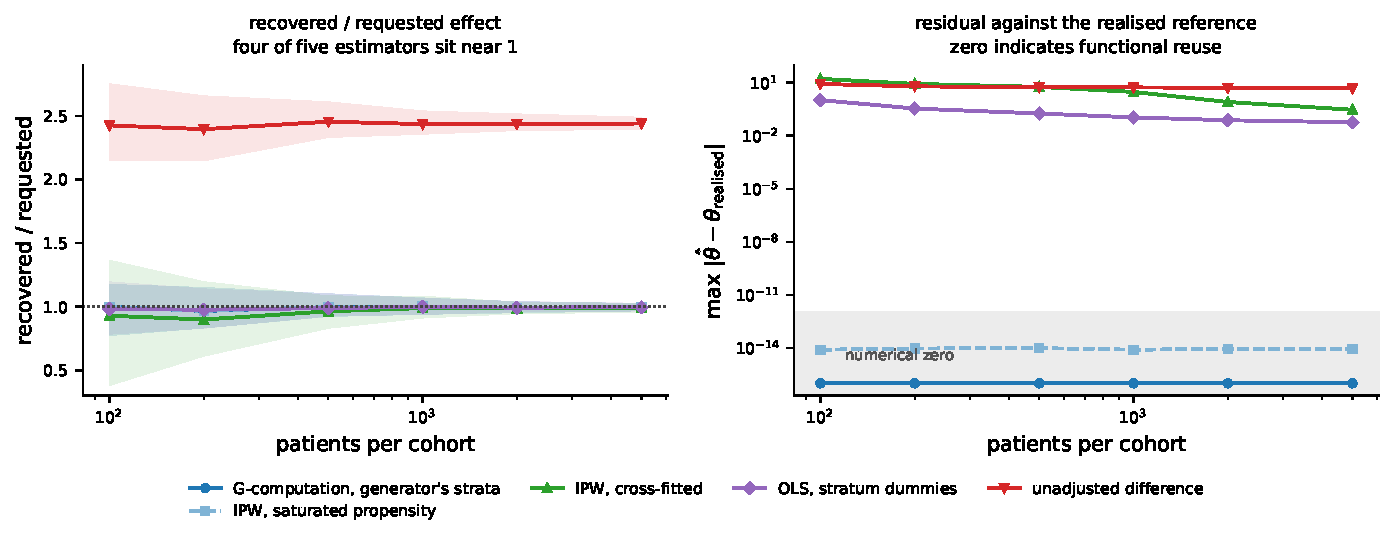
\includegraphics[width=\linewidth]{figures/fig4_trial_recovery.pdf}
\else
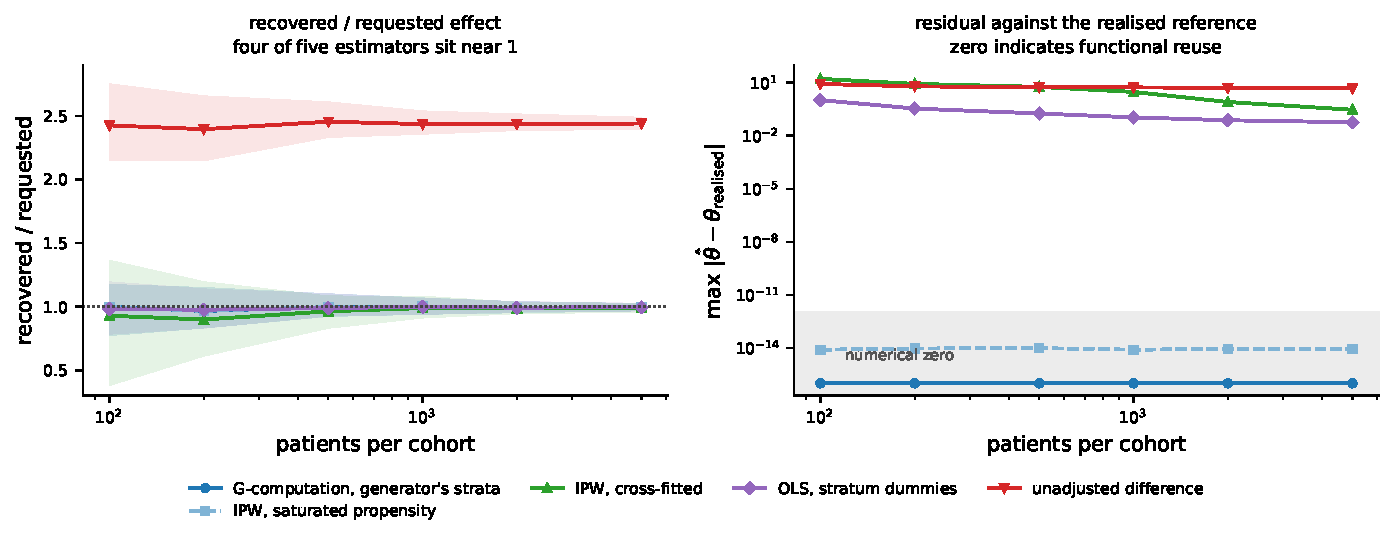
\includegraphics[width=0.88\linewidth]{figures/fig4_trial_recovery.pdf}
\fi
\caption{\textbf{The residual distinguishes reference reproduction from departure.} A patient simulator with confounded assignment and a
requested effect $\theta = 3$. \emph{Left:} recovery curves, median and IQR over
200 replicates (197 at the smallest cohort, where three draws left an arm empty). Four estimators sit near 1 and tighten with cohort size.
\emph{Right:} the residual against the \emph{realised} effect, log scale, shaded
band at machine zero. It is identically zero for G-computation over the
generator's own strata \emph{and for saturated-propensity IPW}, whose curve is
the same line --- both are the same functional of the statistics the generator
drew. Cross-fitted IPW and OLS on stratum dummies are consistent and non-zero, so
they depart from this reference; this does not certify validity. OLS splits
no sample to get there. The unadjusted difference is what a working curve catches.}
\label{fig:trial}
\end{figure}
